\newgeometry{left=4cm, right=2.5cm, top=2.5cm, bottom=2.5cm, marginparwidth=0pt, headsep=0pt}
\chapter{INTRODUCCIÓN}
\pagenumbering{arabic}
\setcounter{page}{1}
% IMPORTANCIA DE MONTAÑA Y PROCESOS HIDROLÓGICOS, PROBLEMATICA DE NO SABER LOS DATOS, PROPUESTA: TLALOCAPP
\section{Contextualización general}

La precipitación es un fenómeno meteorológico que ocurre en sistemas a pequeña escala, caracterizado por la formación de nubes del tipo cúmulus bajo condiciones específicas: presencia de núcleos de condensación, temperaturas cercanas al punto de rocío y un abasto continuo de vapor de agua. A medida que las gotas aumentan de tamaño mediante colisiones, pueden generarse diversas manifestaciones, como lluvia, granizo, nieve, trombas, tornados, rayos y truenos (\cite{ahrens2020}). Complementario a lo anterior, la lluvia se define como la caída de agua procedente de las nubes en estado líquido, sólido y semisólido (\cite{breña2013}). Situándose en regiones montañosas, las condiciones orográficas potencian estos procesos: el relieve obliga a las masas de aire a ascender, condensarse y precipitar, produciendo una mayor captación hídrica que alimenta ríos, acuíferos y sostiene la biodiversidad en zonas bajas (\cite{jiang2003moist, viviroli2007mountain}).

% \section{Importancia hidrológica de las zonas de montaña}



Las zonas de montaña desempeñan múltiples funciones hidrológicas críticas. En primer lugar, actúan como \textbf{fuentes de agua natural}, captando precipitación y alimentando los principales ríos que abastecen a regiones aguas abajo, especialmente en zonas áridas o semiáridas  (\cite{viviroli2007mountain}). Además, la elevación y topografía compleja favorecen procesos de condensación y acumulación de nieve, que posteriormente se transforma en escorrentía estacional  (\cite{immerzeel2020importance}). 

En segundo lugar, estas zonas representan \textbf{reservorios de biodiversidad y hábitats} para especies sensibles al clima, cuya salud está directamente relacionada con la disponibilidad hídrica. También, los suelos y coberturas vegetales en montaña tienen un papel en la regulación del ciclo del agua, facilitando la infiltración y evitando escorrentías extremas  (\cite{buytaert2011mountain}).

% Asimismo, se consideran áreas sensibles al cambio climático, donde las alteraciones en temperatura o precipitación pueden tener consecuencias desproporcionadas sobre la oferta de agua, tanto local como regional  (\cite{beniston2003climatic}). La dinámica hidrológica de estas regiones influye en los servicios ecosistémicos, la agricultura de laderas, y la seguridad hídrica de millones de personas.

% Este estudio, centrado en el monitoreo de precipitaciones mediante ciencia ciudadana en zonas altas como el Monte Tláloc, contribuye indirectamente a la comprensión de estos procesos al generar datos valiosos para validar modelos hidrológicos y climáticos en áreas donde las estaciones meteorológicas tradicionales son escasas o inexistentes.

% PROBLEMAS
Sin embargo, estos ecosistemas de montaña son particularmente sensibles a las alteraciones del clima, lo que los convierte en indicadores clave del cambio ambiental global (\cite{beniston2003climatic}). A nivel mundial, el aumento sostenido de las temperaturas y la recurrencia de eventos extremos están debilitando la estructura y funcionalidad de los bosques, incrementando su mortalidad y reduciendo su resiliencia (\cite{Allen2010}). En México, estas tendencias ya se traducen en mayor aridez y desplazamientos altitudinales de especies forestales. En el Monte Tláloc, por ejemplo, el pino de altura \texttt{Pinus hartwegii} muestra una migración hacia zonas más elevadas, mientras su crecimiento en cotas bajas disminuye, lo cual evidencia un retroceso ante condiciones cada vez más secas (\cite{Astudillo2017}). Esta situación amenaza la cobertura vegetal, la biodiversidad y los servicios ecosistémicos que proveen estos bosques.

Además del cambio climático, los bosques templados de montaña enfrentan presiones como la deforestación y la fragmentación del hábitat. Estos factores, sumados a la limitada cobertura de estaciones meteorológicas en zonas remotas, dificultan una adecuada medición de la precipitación, especialmente en regiones de difícil acceso como el Monte Tláloc (\cite{aparicio1992}). Por lo tanto carencia de datos de precipitación compromete los esfuerzos de conservación y gestión forestal sustentable (\cite{hernandez2021}).
% SOLUCIÓN: CIENCIA CIUDADANA
Ante este panorama, la ciencia ciudadana emerge como una herramienta innovadora y una solución para el monitoreo climático. Esta estrategia permite que personas no expertas contribuyan en la recolección, validación y análisis de datos ambientales, mejorando la resolución espacial y temporal de la información disponible (\cite{csic_ciencia_ciudadana, viegas2023citizen, elmore2014mping, lei2022combining}). En particular, el monitoreo ciudadano de lluvias ha demostrado ser eficaz para capturar eventos localizados que escapan a las redes oficiales, además de fomentar el conocimiento climático local y la resiliencia comunitaria frente a eventos extremos (\cite{okada2019community, ciga_monitoreo}).

El presente trabajo propone el desarrollo de un paquete tecnológico que promueva la participación ciudadana en el monitoreo de precipitaciones en zonas de montaña, tomando como caso de estudio el Monte Tláloc. Los objetivos específicos son: (1) definir un protocolo de monitoreo participativo funcional y confiable, con pluviómetros distribuidos estratégicamente; (2) diseñar e implementar una aplicación digital multiplataforma con interfaz intuitiva para registrar, visualizar y compartir datos meteorológicos; y (3) evaluar el nivel de madurez tecnológica del sistema utilizando la escala internacional Technology Readiness Levels (TRL), estimando su viabilidad en condiciones reales.


\section{Planteamiento del problema}

Ante la falta de datos sobre precipitación en estas zonas, se requiere el desarrollo de estrategias innovadoras que permitan superar las limitaciones técnicas y logísticas, involucrando a las comunidades locales en la generación y uso de información. Es necesario recurrir a estrategias que incorporen a la población en la generación de información y en su utilización para el manejo de los ecosistemas (\cite{hubp1990}).


En México, las redes oficiales de monitoreo hidrometeorológico, como las operadas por la Comisión Nacional del Agua (CONAGUA), presentan una cobertura limitada en muchas regiones de montaña, donde los microclimas pueden variar significativamente en distancias cortas (\cite{rosas2021}).


El Monte Tláloc, ubicado en la zona montañosa del oriente del Valle de México, es un ejemplo de ello: su importancia ambiental, histórica y cultural contrasta con la escasa información climática precisa y en tiempo real disponible para la comunidad local, investigadores y tomadores de decisiones. Esta falta de datos puntuales dificulta la gestión sustentable del agua, la prevención de riesgos y el análisis del cambio climático a escala local.

Las aplicaciones disponibles para la recolección de datos meteorológicos suelen ser de uso profesional, poco accesibles o no están diseñadas para fomentar la participación ciudadana en contextos rurales o de baja conectividad. Esto genera una brecha entre el potencial de colaboración ciudadana y las herramientas disponibles para lograrlo.

Ante este panorama, surge la necesidad de desarrollar una aplicación multiplataforma intuitiva, accesible y robusta, que aproveche el poder de la ciencia ciudadana para llenar los vacíos de información sobre la precipitación en el Monte Tláloc. Dicha aplicación debe facilitar la recolección, visualización y validación de datos por parte de usuarios no expertos, promoviendo la generación de conocimiento colectivo, la educación ambiental y la participación de la comunidad en temas de gestión hídrica y climática.


\section{Justificación}
Se identifica la necesidad de crear un instrumento para la captura y envío de datos pluviales que sea accesible, participativo y que garantice la disponibilidad de la información obtenida para su análisis y toma de decisiones. Este instrumento debe ser sencillo de usar y estar diseñado específicamente para el público objetivo. Ellos, a través de su participación activa, pueden convertirse en aliados estratégicos para la recolección continua de datos.

La aplicación desarrollada se plantea como una solución innovadora que responde a esta necesidad. Su diseño intuitivo permite que usuarios con conocimientos tecnológicos básicos puedan capturar y enviar información sobre las precipitaciones de manera rápida y eficiente. Además, al integrar elementos de ciencia ciudadana, se fomenta la colaboración activa de las comunidades locales, fortaleciendo su empoderamiento y compromiso con la conservación de los recursos naturales. Desde un enfoque técnico, el proyecto destaca por su carácter práctico y adaptable.

La app aprovecha tecnologías modernas para registrar datos de lluvia, optimizando la recopilación de información en tiempo real, y reduciendo costos asociados a equipos de medición tradicionales. Al centralizar y analizar estos datos en una plataforma digital, se genera un repositorio de información confiable que puede ser utilizado por investigadores, autoridades locales y los mismos ejidatarios para tomar
decisiones fundamentadas.

Por último, la disponibilidad de esta información en un formato accesible y visualmente comprensible contribuye a sensibilizar a los usuarios sobre la importancia de monitorear los patrones de lluvia, facilitando su uso en estrategias de manejo hídrico, planificación y mitigación de riesgos climáticos. De esta forma, el proyecto no solo pretende solucionar un problema técnico, sino que también puede tener un impacto social y ambiental significativo.



% \section{Hipótesis}
% \subsection{Hipótesis general (H)}

% La implementación de una aplicación multiplataforma basada en ciencia ciudadana incrementa significativamente la frecuencia y precisión de los reportes de lluvia en la región del Monte Tláloc, al promover la participación de los habitantes locales mediante herramientas digitales accesibles. Esto permite generar información meteorológica complementaria a la de las estaciones profesionales, mejorando la caracterización espacial y temporal de los eventos de precipitación.


% \subsubsection{Hipótesis nula ($H_0$)}
% La implementación de una aplicación multiplataforma basada en ciencia ciudadana \textbf{no tiene un efecto significativo} en la frecuencia ni en la precisión de los reportes de lluvia en la región del Monte Tláloc, ni contribuye sustancialmente a la caracterización de los eventos de precipitación.

% \subsubsection{Hipótesis alternativa ($H_1$)}
% La implementación de una aplicación multiplataforma basada en ciencia ciudadana \textbf{sí mejora significativamente} la frecuencia y precisión de los reportes de lluvia en la región del Monte Tláloc, y contribuye a una mejor caracterización de los eventos de precipitación respecto a los datos generados únicamente por estaciones profesionales.

\section{Alcance de la tesis}

Esta tesis se enmarca en del desarrollo tecnológico aplicado al monitoreo climático participativo en zonas rurales de difícil acceso. En particular, se concentra en el diseño, implementación y validación de una aplicación multiplataforma basada en principios de ciencia ciudadana, con el objetivo de mejorar la frecuencia, cobertura y trazabilidad de los reportes de lluvia en la región del Monte Tláloc.

El alcance del trabajo está delimitado a un protocolo de monitoreo participativo validado con las comunidades locales; la creación de un sistema funcional compuesto por una herramienta digital (Tláloc App); y una primera aproximación del estado del nivel tecnológico. No se abordan en esta tesis predicciones climáticas avanzadas, análisis hidrológicos derivados ni su integración con sistemas nacionales meteorológicos, aunque se plantean como trabajo futuro.

Con base en lo anterior, esta investigación abarca los siguientes logros concretos:

\begin{itemize}
  \item \textbf{Demostración técnica de la viabilidad.} Se valida que es posible registrar mediciones meteorológicas confiables mediante dispositivos móviles de bajo costo y pluviómetros, sin requerir formación técnica previa por parte de los usuarios. Un pluviómetro manual es un instrumento utilizado para medir la cantidad de precipitación líquida caída en un lugar específico durante un período determinado. Consiste en un recipiente cilíndrico que recoge el agua de lluvia, la cual se mide posteriormente con una probeta graduada. Este instrumento debe cumplir con las especificaciones establecidas en las normas mexicanas para garantizar la precisión y confiabilidad de los datos obtenidos (\cite{semarnat_pluviometro}). Las especificaciones para construir un pluviómetro son las siguientes:%(Figura \ref{t1}), son las siguientes:
\begin{itemize}
    \item El depósito debe tener una entrada estrecha, suficientemente protegida de la radiación, para reducir al mínimo las pérdidas de agua por evaporación.
    \item Este instrumento debe colocarse en lugares abiertos y su área de captación debe permanecer horizontal y a 100 cm del suelo (\cite{se2013}).
\end{itemize}

% \begin{figure}[h!]
% \centering
%   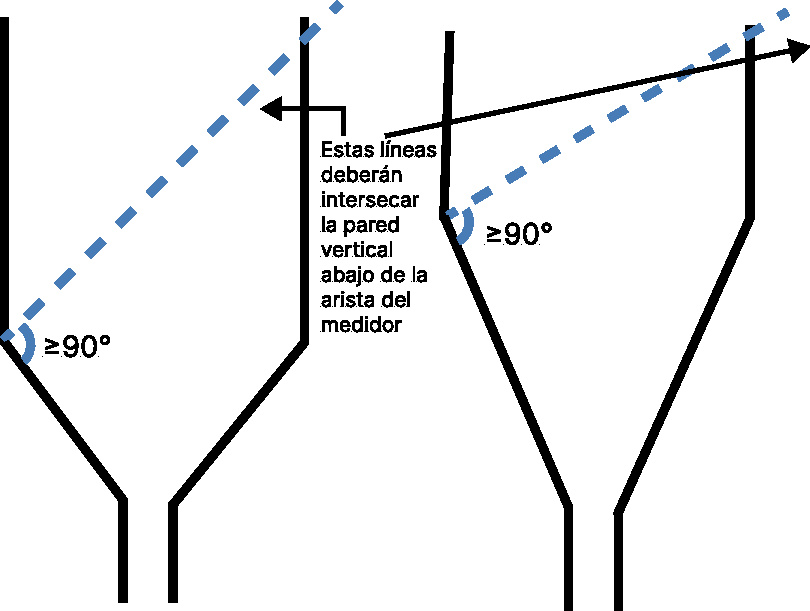
\includegraphics[width=0.5\textwidth]{t1.pdf}
%   \caption{Colectaros adecuados para los pluviómetros según la norma NMX-AA-166/1-SCFI-2013 (\cite{se2013})}
%   \label{t1}
% \end{figure}
  
  \item \textbf{Desarrollo de programa de cómputo con una arquitectura modular y escalable.} Se implementa una aplicación desarrollada en Flutter que permite su ejecución en múltiples plataformas (Android y Web), integrando servicios en la nube como Firebase para autenticación, almacenamiento y sincronización en tiempo real.
  
  \item \textbf{Trazabilidad.} Cada medición capturada incluye coordenadas geográficas y marcas temporales, lo que permite realizar análisis espaciales y temporales sobre la distribución de la lluvia.
  
  \item \textbf{Visualización y exportación de datos.} Se incluyen herramientas gráficas interactivas, filtros temporales y funciones de exportación en formatos como Excel y PDF, pensadas para su integración en informes técnicos o investigaciones científicas.
  
  \item \textbf{Evaluación de madurez tecnológica.} El prototipo fue probado exitosamente en condiciones reales con usuarios de la comunidad del Monte Tláloc, alcanzando un nivel de madurez tecnológica estimado en TRL 8, correspondiente a una solución validada y comercializable.
\end{itemize}

Este estudio representa un esfuerzo interdisciplinario que combina ingeniería de software, participación comunitaria y gestión ambiental, proponiendo una metodología replicable para la generación participativa de datos meteorológicos en regiones donde los sistemas tradicionales no tienen cobertura.




\section{Organización de la tesis}

Este documento está estructurado de acuerdo con el proceso integral de investigación, desarrollo y validación de una aplicación multiplataforma orientada a la ciencia ciudadana, enfocada en el monitoreo de precipitaciones en el Monte Tláloc. La redacción mantiene una notación consistente en todo el texto, con excepciones claramente indicadas cuando es necesario. Al final del documento se presenta una bibliografía acumulativa con todas las referencias consultadas.

\begin{itemize}
    \item \textbf{Capítulo 1: Introducción.} Presenta el planteamiento del problema, el contexto geográfico del Monte Tláloc, la justificación del proyecto, el esquema general del documento y las limitaciones del estudio.
    
    \item \textbf{Capítulo 2: Objetivos.} Define el objetivo general y los objetivos específicos que guiaron la realización del presente trabajo de investigación y desarrollo tecnológico.
    
    \item \textbf{Capítulo 3: Revisión de literatura.} Sistematiza los conceptos clave necesarios para comprender el proyecto, incluyendo el acceso a datos meteorológicos en zonas montañosas de México, experiencias previas en monitoreo ciudadano, tecnologías digitales aplicadas al monitoreo climático, y el papel de la ciencia ciudadana en el estudio ambiental.
    
    \item \textbf{Capítulo 4: Materiales y Métodos.} Detalla los recursos físicos empleados, la arquitectura tecnológica implementada, el protocolo de monitoreo participativo validado, el proceso de desarrollo de la aplicación Tláloc App y la metodología utilizada para estimar su nivel de madurez tecnológica.
    
    \item \textbf{Capítulo 5: Resultados.} Presenta la estrategia detallada y justificada de un protocolo de monitoreo replicable; el desempeño funcional de la aplicación y el llenado del formulario de la evaluación, obteniendo el nivel de desarrollo tecnológico (TRL).
    
    \item \textbf{Capítulo 6: Conclusiones y trabajo futuro.} Resume los aportes de la tesis al campo del monitoreo ambiental, las principales contribuciones de la tesis, plantea escenarios de expansión hacia otras regiones y propone líneas futuras de desarrollo.
\end{itemize}


